\documentclass[a4paper]{article}

\usepackage[english]{babel}
\usepackage[utf8]{inputenc}
\usepackage{graphicx}


\title{Virtual Reality: A Study in Immersion}

\author{Daniel Levine}

\date{\today}

\begin{document}
\maketitle

\begin{abstract}
\indent \indent This paper is a comprehensive study of both the Oculus Rift and Microsofts RoomAlive project, and their ?immersiveness?. The paper explores a brief history of virtual reality and the potential for both devices. It will also go over the mental models and usability issues in of both the devices. The study determines that Oculus Rift seems to be the future in regard to immersive technology. 

\end{abstract}

\section{Introduction}

\indent \indent Screens have seen major advancements in recent years with the technology of HD TVs to LED to 3D, and most recently Ultra High Definition (or 4k). Through these changes, it seems that the mental model of the creators has been to deliver a more immersive experience. This can be demonstrated by the creation of the new curved TV by Samsung, or the recent rise in the use of projectors in homes to make screens so big, that it feels like you're in the room with what is going on in the screen. The goal of complete immersion seems to be leading eventually toward holograms, (3D imagery not requiring a screen), and virtual reality, (?a computer-generated simulation of a three-dimensional image or environment that can be interacted with in a seemingly real or physical way by a person using special electronic equipment, such as a helmet with a screen inside or gloves fitted with sensors")\cite{1}) so that a TV isn?t even necessary anymore. Steps toward complete immersion are already being taken with the Oculus Rift and Sony's Morpheus Project. Both are virtual reality headsets that allow the user to feel as if they are in the game, by cutting out all distractions like noise and peripheral vision. On the other side of the immersion spectrum, Microsoft?s response to virtual reality is their prototype called RoomAlive, which they use kinect devices attached to projectors in order to turn the whole room into an interactive environment. It gives the user a different sense of immersion. These two examples show two very different ways that the researchers are trying reach the nearly graspable task of complete immersion. On one side of the spectrum with the Oculus Rift, they are trying to achieve total immersion by cutting you off from the outside world, hence limiting possible distractions from what is going on in the screen. Whereas on the other side, Microsoft's RoomAlive project brings the program to you making your entire room a holodeck of sorts. These examples highlight the differences in the mental models between these two up and coming technologies. This battle between virtual reality and holograms seems to be the future for screens, however both are not without faults especially from a usability standpoint.


\section{Background/Prior Work/Literature Review}


\indent \indent Virtual Reality isn?t as new an idea as most people believe. The idea of a virtual reality headset can originate itself to the 1930s book ``Pygmalion's Spectacles'' by Stanley G. Weinbaum \cite{1}. In the 1990s sega came out with virtual reality headsets, however, Virtual Reality technology at the time suffered from a myriad of usability issues at the forefront of which was motion sickness as ?the onscreen graphics didn?t keep pace with the gamer?s head movements?\cite{2}.The Oculus Rift has been able to eventually overcome these issues that had previously been the demise of its predecessors by ?reducing the lag between head movement and the headset response to just 2 milliseconds?\cite{2}. Although there will most likely always be a small subset of people where the issue of motion sickness remain, this  innovation has made virtual reality on a more widespread scale possible.\\

\indent The creator of the Oculus Rift, Palmer Lucky, made it as a way to ?bring games to the next level? by his method he called ?plugging into the matrix?. He achieved this by using ?immersive stereoscopic 3d rendering, a massive field of view and ultra low latency head tracking?\cite{3}. When using most stereoscopic headsets you see ? a really small image way off into the distance?, whereas with the Oculus Rift you get a view of 110 degrees making it seem as if you are in the environment\cite{3}.This was Lucky?s way of sharing his vision of a new completely immersive technology with possible developers and consumers.\\
\indent In a recent study, a youth research and digital entertainment firm gave 12 children, ages 7 to 12, the Oculus Rift to use. The study had extremely positive results. They found that ?while the children had some trouble getting the headset on, the kids did not have any ill effects from wearing it for too long, but noted that the head movements could be a strain on younger players?\cite{4}, however, the study goes on to note that with lighter headsets on the way they don?t see many usability issues with the Oculus Rift especially in children.\\
\indent Another study conducted in 2013 by Adam Halley-Prinable, a graduate student at Bournemouth University, studied the immersiveness of an Oculus Rift device as opposed to a standard computer monitor. In order to do this, he created ?an original horror game created by the author?, and measured ?the immersiveness through fear that the Oculus Rift caused? and compared it to "the immersiveness that the screen caused?\cite{7}. The study measured fear by using a heart rate test and found that increased immersion leads to increased fear, ? This means that in a controlled environment, a measurement of fear is a measurement of immersion?\cite{7}. 
Each test subject was booked into a 30 minute timeslot, ?altogether 56 of the total 60+ people who participated in this experiment were able to contribute their data?\cite{7}. Some of the subjects were unable to finish the game because ?overwhelming psychological anguish and terror, while others still were unable to complete the Oculus Rift section because of induced headaches, nausea, and dizziness?\cite{7}. The study found that of the ?56 people who completed the questionnaire fully, 2 people found the screen more immersive, 3 people found both options equally immersive, and the remaining 51 people found the Oculus Rift to be the most immersive.?\cite{7}\\
\indent Creators of RoomAlive call the technology ?projection mapping?. It is meant to turn a room into ?an immersive, augmented entertainment experience through the use of video projectors?\cite{6}.The RoomAlive project was built mainly off of one of Microsoft's previous projects, ?IllumiRoom, which explored interactive projection mapping surrounding a television screen?\cite{6}. The place where RoomAlive differs from IllumiRoom is that IllumiRoom ? was largely focused on display, extending traditional gaming experiences out of the TV?\cite{6}. RoomAlive focuses more on ?interaction, and the new kinds of games that we can create with interactive projection mapping?\cite{6}. In order to do all this, they use what they call a ?procam?, which is essentially a projector connected to a Kinect sensor. The Kinect is used for tracking, while the projector is for display.


\begin{figure}
\centering
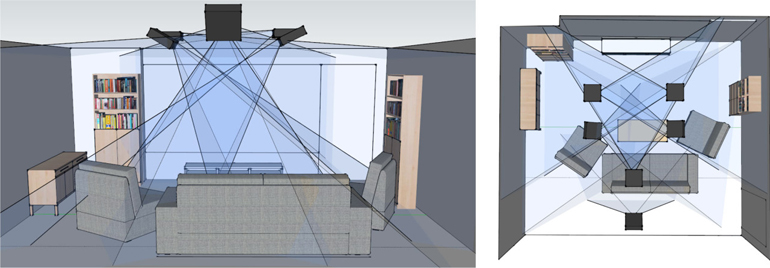
\includegraphics[scale=0.4]{roomalive.jpg}
\caption{RoomAlive concept}
\end{figure}



\section{Methods}

\indent\indent Technological information for both Oculus and RoomAlive were collected from numerous studies, articles, and forums. For this study, I tried to obtain the data from a recently conducted survey\cite{8} by a student at the University of Glasgow. However, he was unable to release the results until the paper is published. Of the information in this paper, the one of most relevance is the study of that pits the Oculus Rift against the standard monitor, as a way to determine which is ultimately more immersive. This study seems to hold weight due to its large sample size and extremely positive results based on the data collected. The paper also shows that the Oculus Rift has faired well when tested particularly when it is being tested for immersion.

\section{Discussion}


\indent \indent The technology of Virtual Reality has grown leaps and bounds leading to the creation multiple new devices, the most prevalent one being the Oculus Rift. Public support for virtual reality technology was made evident during the original kickstarter campaign for the Oculus Rift, initially requesting funding of 250,000 dollars. The project received close to 10 times that amount before it was bought by Facebook for 2 billion dollars. The clear mental model that the creator of the Oculus Rift, Palmer Lucky, was to change the way that people play games by creating a "truly immersive virtual reality"\cite{3}, a mental model he hoped to translate to users through the medium of his device, the Oculus Rift. One of the usability issues that had made this difficult in the past with other stereoscopic headsets had been the weight of the screen, making it hard to move around. The sensors that track your head movement have gotten much better. The results found in the study by Dubit Limited where the children tested the Oculus Rift, were in overwhelming support of the Oculus Rift?s usability particularly in children. The study came to a few interesting conclusions. For example, the games that were grounded in reality performed much better than the games that we based on abstract concepts. The research done by Adam Halley-Prinable interestingly found that fear and immersion didn?t correlate when using the Oculus Rift, even though the users found the Oculus Rift both more ?scary and immersive?\cite{7}. The experiment did find usability issues with the Oculus Rift with some users being unable to finish because of dizziness nausea or  headaches.\\
\indent Other usability issues that still plague the Oculus Rift are mainly revolving around interaction with reality. Finding your keyboard or controller with the headset on could potentially lead to problems if the space near your keyboard or controller is not kept clean, or if you have other objects in the area. Another potential problem could be that if you are in the room with someone else, the headset effectively limits all interaction with the people in your immediate vicinity. Students at the University of Glasgow have recognized usability issues and have even gone as far as prototyping possible solutions for them(see video\cite{5}). However, it seems these usability issues are simply a byproduct of Palmers initial mental model, and perhaps may be a necessary evil to provide a ?truly immersive virtual reality? experience\cite{3}.\\ 
\indent The competition to the new age of virtual reality headsets coming out is one that takes a different stance on how virtual reality should be displayed, with the introduction holographic environments. The mental model the creators of RoomAlive have in mind is the creation of an ?Immersive augmented experience?  that ?transforms the room into a new (Interactive)environment?\cite{6}. Microsoft?s RoomAlive project, still in developmental stages, represents the alternative to stereoscopic headsets, while being very reminiscent to Star Trek?s holodeck. While RoomAlive is still in its early developmental stages, I can see a multitude of usability problems arising with this initial concept. One of which would be the possibility of running into objects while using the RoomAlive, because the RoomAlive could potentially obstruct your view of other objects around the room. Another problem that could potentially doom the RoomAlive project is cost, the IllumiRoom project was initially ended because it was deemed ?too expensive for consumers? \cite{6}. Even though it may not be a usability issue, it seems that the RoomAlive may also fall to the same fate of its predecessor based on the fact that it relies on 6 procams to Illumiroom's 1 procam. While the concept might be on the right track, it seems to be a while till the RoomAlive projects mental model will be able to connect to users.


\begin{figure}
\centering
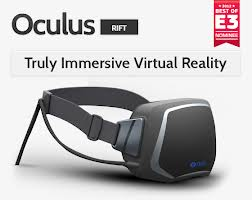
\includegraphics[scale=0.4]{OculusRift.jpg}
\caption{Oculus Rift}
\end{figure}





\section{Conclusion}

\indent \indent As we can see from the studies conducted, the Oculus Rift has had exceptional results when tested for immersion as the possiblities for it continue to grow. The mental model of a "truly immersive virtual reality"\cite{3} expierience seems to be become a reality for Palmer Lucky and the people who worked on the Oculus Rift, while RoomAlive still has some hurdles to overcome before it can be seen as anything other than just a concept. 


\section{Cognitive Psychology Questionnaire}

\subsection{Question 1}
Give at least two specific examples of objects or behaviors that cognitive psychologists study.\\

Two specific behaviors that cognitive psychologists study are Handedness and Emotion.

\subsection{Question 2}
How do these subjects of study relate to what interaction design studies?\\

These subjects can make for much improved designs. For example the study of emotion can help make programs evoke an expected reponse from people.

\subsection{Question 3}
Give at least 2 specific methods used by cognitive psychologists to study or learn about their subjects.\\

One method that congnitive psychologists use to study subjects is to study split brain patients to get a better understanding of the hemisphere of the brain. Another method is to take a picture and make it symmetrical and see what emotional response it ellicts from the patient.  

\subsection{Question 4}
How do these methods of study relate to how interaction design reaseach is performed?\\

These methods can help guide interaction design reasearch by helping designer improve his mental model to cater more to the users mental model.


\begin{thebibliography}{9}

\bibitem{1}
"Virtual Reality."Wikipedia. Wikimedia Foundation, 19 Oct. 2014.Web. 21 Oct. 2014.

\bibitem{2}
Barras, Colin.
"How Virtual Reality Overcame Its ?puke Problem?." BBC Future.BBC, 27 Mar. 2014.Web.10 Oct. 2014

\bibitem{3}
"Oculus Rift: Step Into the Game."Kickstarter. N.p., n.d. Web. 10 Oct. 2014.
  
\bibitem{4}  
Robinson, Peter. "Researching Oculus Rift with Kids: What They Really Think of Virtual Reality." Dubit Limited. Dubit Limited, 24 June 2014. Web. 10 Oct. 2014

\bibitem{5}
 McGill, Mark. "Augmented Virtuality Prototypes." YouTube. YouTube, 3 Sept. 2014. Web. 21 Oct. 2014.
 
\bibitem{6}
Jones, Brett. "RoomAlive: Magical Experiences Enabled by Scalable, Adaptive Projector-Camera Units." Http://projection-mapping.org/. N.p., 8 Oct. 2014. Web. 13 Oct. 2014.

\bibitem{7}    
Halley-Prinable, Adam. "The Oculus Rift and Immersion through Fear. "Http://www.academia.edu/. Bournemouth University, Sept. 2013. Web. 13 Oct. 2014.  
  
\bibitem{8}
McGill, Mark. "Oculus Developer Forums." Survey on Usability. N.p., 01 Sept. 2014. Web. 05 Oct. 2014.  

\end{thebibliography}




\end{document}